\newpage
\chapter{表格}
\thispagestyle{chapterpage}

\section{浮动体}

在学习\LaTeX{}表格和图片的编排之前,了解一下什么是浮动体。\textbf{图片和表格有时会很大,在插入的位置不一定放得下,因此需要浮动调整,这样一个浮动调整的环境就成为浮动体。}

\note{因为有浮动体的存在,图片编排的位置是不确定的,所以要避免在文中使用「下图」、「上图」的说法,而是使用ref命令生成图表的编号。}

浮动体将图或表与其标题定义为整体,然后动态排版,以解决图、表卡在换页处造成的过长的垂直空白的问题。但有时它也会打乱你的排版意图,因此使用与否需要根据情况决定。图片的浮动体是figure环境,而表格的浮动体是table环境。

对表格来说,输出表格内容的是tabular环境,\textbf{table}只是一个会浮动体(到处乱跑的盒子)而已。没有tabular环境,table环境一样会乱跑;没有table环境,tabular环境一样会输出表格内容。图片浮动体与表格是一样的。图片和表格的浮动体环境如下所示:

\begin{latex}
\begin{table}[!htbp]
表格
\end{table}
%%%%%%%%%%%%%%%%%%%%
\begin{figure}[!htbp]
图片
\end{figure}
\end{latex}

!表示忽略内部参数(比如内部参数对一页中浮动体数量的限制);h当前位置(here),t顶部(top),b底部(bottom),p单独成页(p)。\LaTeX{}的默认参数是tbp。另外需要注意的是label命令写在caption命令下方,否则交叉引用会出现问题。

\section{array宏包}

数组宏包\emph{array}改进和扩展了\LaTeX 的\emph{tabular、tabular*、array}环境的功能,增强了\emph{列格式}的功能和一些其他表格参数的调整功能。

\begin{table}[!htb]
    \centering
    \caption{array宏包基本参数}
    \begin{tabular}{ll}
    \toprule
    选项 & 说明 \\
    \midrule
    l & 左对齐 \\
    c & 居中 \\
    r & 右对齐 \\
    p\{列宽\} & 顶对齐 \\
    m\{列宽\} & 居中对齐 \\
    b\{列宽\} & 底对齐 \\
    @\{声明\} & 该列每行都插入声明中的文本 \\
    >\{声明\} & 命令或需要插入列元素前的文本 \\
    <\{声明\} & 命令或需要插入列元素后的文本 \\
    | & 在列边或列间插入垂直线 \\
    !\{声明\} & 在列间插入声明要求的样式 \\
    \bottomrule
    \end{tabular}
\end{table}

\section{booktabs宏包}

这个宏包是用来专门排版三线表的。其形式简洁、功能分明、阅读方便,广泛用在科技论文写作中排版实验测量和计算数据。\pkg{booktabs}宏包就是一个非常适合用来排版三线表的宏包。用法非常简单,代码如下,\autoref{SHB}是一个三线表示例。

\begin{latex}
\begin{tabular}{lll}
    \toprule[2pt]
    表格内容
    \midrule[0.5pt]
    表格内容
    \bottomrule[0.5pt]
\end{tabular}
\end{latex}

其中,每个表格只有一条toprule和bottomrule,但midrule可以添加任意多。

\begin{table}[!htb]
    \caption{Ozone decomposition of SHB mechanism}
    \label{SHB}
    \centering
    \begin{tabular}{lll}
        \toprule[2pt]
        State & Equation & Reaction rate constant\\
        \midrule[0.5pt]
        Chain initiation & \ce{O3 + OH- -> HO2* + O2*} & $k_1 = \SI{70}{L/\mole \cdot \second}$\\
        Chain transfer & \ce{HO2* -> O^{-}_2 * + H+} & $k_2=\SI{7.9e5}{L/(\mole \cdot \second)^{25}}$\\
        & \ce{O^{-}_2 * + H+ -> HO_2 *} & $k_3=\SI{5e10}{L/(\mole \cdot \second)^{25}}$\\
        & \ce{O3 + O^{-}_2 * -> O^{-}_3 * +O2} & $k_4=\SI{1.6e9}{L/(\mole \cdot \second)}$\\
        & \ce{O^{-}_3 + H+ -> HO3 *} & $ k_5=\SI{5.2e10}{L/(\mole \cdot \second)} $\\
        & \ce{HO3* -> O^{-}3 + H+} & $ k_6=\SI{3.3e2}{\second^{-1}} $\\
        & $ \cdots $ & $ \cdots $ \\
        Chain termination & \ce{HO4 * +HO4 * -> H2O2 * +2O3} & $ k_{10}=\SI{5e9}{L/(\mole \cdot \second)^{25}} $\\
        & \ce{HO4* + HO3* -> H2O2* + O2 +O3} & $ k_{11}=\SI{5e9}{L/(\mole \cdot \second)^{25}} $\\
        \bottomrule[0.5pt]
    \end{tabular}
\end{table}

\lstinline|\cmidrule|能用来画局部水平线,可以用来制作跨列表格。局部水平线可以有多条,但需要在其他cmidrule前添加\lstinline|\morecmidrules|命令,否则多条局部水平线重叠为一条。

\begin{table}[!htb]
    \centering
    \caption{Weather statistics}
    \begin{tabular}{cccc}
        \toprule[2pt]
        & \multicolumn{3}{c}{weather}\\
        \cmidrule{2-4}
        \morecmidrules\cmidrule{2-4}
        months & rain & sunny & cloudy\\
        \midrule
        1 & 2 & 1 & 0\\
        \midrule
        \addlinespace[5pt]%增加某一行高度
        2 & 3 & 2 & 1\\
        \addlinespace[5pt]
        \bottomrule
    \end{tabular}
\end{table}

\section{表格}
\LaTeX 原生的表格功能非常有限,甚至不支持单元格跨行和表格跨页,我们必须通过宏包来解决。如有需求,可在\emph{tabular}环境外定义全部表格线的粗细,例如,\lstinline|\setlength{\arrayrulewidth}{2pt}|或者直接写\lstinline|\arrayrulewidth=2pt|。

\begin{codeshow}
\centering
\arrayrulewidth=1pt%表格线宽度
\begin{tabular}
    {|c|c|c|}
    \hline
    \multicolumn{3}{|c|}{整体表格线宽}\\
    \hline
    7 & 5 & 3 \\
    \hline
    6 & 1 & 8 \\
    \hline
\end{tabular}
\end{codeshow}

如果需要单独定义某一条表格线的粗细,必须要做额外的设置。比如我们要更改垂直表格线的粗细,可以利用array宏包提供的新列格式选项定义命令。其中的新选项名只能用一个字母来表示。使用该命令更改中间两条垂直线粗细为2pt。

\begin{latex}
\newcolumntype{新选项名称}[参数数量]{列格式}
\newcolumntype{I}{!{\vrule width 4pt}}
\end{latex}

\begin{codeshow}
\centering
\newcolumntype{I}{!{\vrule width 2pt}}
\begin{tabular}
    {|c|c|c|}
    \hline
    \multicolumn{3}{IcI}{垂直线粗细}\\
    \hline
    7&5&3\\
    \hline
    6&1&8\\
    \hline
\end{tabular}
\end{codeshow}

水平表格线的粗细较难修改,需要使用booktabs宏包,该宏包可以任意修改水平线粗细,还可以在其上、下方附加一段垂直空白。

\begin{codeshow}
\centering
\begin{tabular}
    {|c|c|c|}
    \hline 
    \multicolumn{3}{|c|}{水平线宽}\\
    \specialrule{2pt}{0pt}{0pt}
    7&5&3\\
    \hline
    6&1&8\\
    \hline
\end{tabular}
\end{codeshow}

\emph{array}包重新实现了\emph{tabular}环境,加了不少新选项进去。比如我们可以定义\emph{F}为一个居中且在数学环境中的列类型。然后在\emph{tabular}中调用\emph{F}即可在表格环境中排出数学样式。

\begin{codeshow}
\newcolumntype{F}{>{$}c<{$}}
\centering
\begin{tabular}{FFF}
    \alpha & \beta    & \gamma   \\
    \delta & \epsilon & \upsilon \\
    \sigma & \tau     & \phi     \\
\end{tabular}
\end{codeshow}

\subsection{跨行和跨列表格}

\cmdindex{multirow}
\cmdindex{multicolumn}

既跨行又跨列时,必须把\lstinline|\multirow{number of rows}{width}{text}|命令放在\lstinline|\multicolumn{code}{pos}{text}|内部,始终记住\textbf{跨列享受最高的优先级}。

\begin{codeshow}
\centering
\begin{tabular}{|c|c|c|}
    \hline
    \multirow{2}{*}{跨行} & \multicolumn{2}{c|}{跨列} \\ \cline{2-3}
     & abc & 123 \\ \hline
    \multicolumn{2}{|c|}{\multirow{2}{*}{跨行跨列}} & XYZ \\ \cline{3-3}
    \multicolumn{2}{|c|}{} & xyz \\ \hline
\end{tabular}
\end{codeshow}

\begin{codeshow}
\centering
\begin{tabular}{|ccc|}
    \hline
    2 & 9 & 4 \\
    7 & \multicolumn{2}{c|}{\multirow{2}{*}{?}}\\
    6& & \\ \hline
\end{tabular}
\end{codeshow}

\subsection{彩色表格}

利用\pkg{xcolor}宏包的颜色功能,\pkg{colortbl}宏包上给表格上色。提前定义好所需要的颜色。

\begin{latex}
%表格颜色
\definecolor{oddrows}{RGB}{243,246,246}%奇数行
\definecolor{evenrows}{RGB}{228,228,228}%偶数行
\definecolor{header}{RGB}{0,104,183}%表头
\end{latex}

使用\lstinline|\rowcolor{color}|单独给某一行行上色,使用xcolor宏包提供的\lstinline|\rowcolors{start}{oddrows}{evenrows}|快速设定奇偶行颜色。\LaTeX{}毕竟是做科技排版的,太花哨的彩色表格没有多大意义,用\LaTeX{}做起来也难受,不要深究。\autoref{color-tabular}~这种表头设定深色,奇偶行颜色交替的表格在科技排版中应用较多。

\begin{table}[!htb]
    \centering
    \caption{彩色表格演示}
    \label{color-tabular}
    \rowcolors{2}{oddrows}{evenrows}
    \begin{tabular}{ccc}
        \rowcolor{header}
        \color{white} \textbf{姓名} &\color{white} \textbf{学号} &\color{white} \textbf{性别}\\
        张三 & 2016121 & Male\\
        李四 & 2016122 & Male\\
        王五 & 2016123 & Male\\
        赵六 & 2016124 & Male\\
    \end{tabular}
\end{table}

\subsection{斜线表头}

虽然斜线表头是不符合国标的,但在非正式场合用得还挺多的。制作斜线表头需要\pkg{diagbox}宏包,刘海洋写的,中文说明。

\begin{codeshow}
\centering
\begin{tabular}{|l|ccc|}
    \hline
    \diagbox{Time}{Room}{Day}
        &Mon&Tue&Wed\\
    \hline
    Morning&used&used&\\
    Afternoon& &used&used\\
    \hline
\end{tabular}
\end{codeshow}

\subsection{表格标题}

表格标题命令默认只能在浮动体内使用,在导言中添加如下命令,便可以在浮动体外使用\verb|\figcaption|和\verb|\tabcaption|命令来为图标添加标题。为了防止标题和图表不在一页,我们也可以用\verb|minipage|环境把它们包起来。

\begin{latex}
\makeatletter
\newcommand\figcaption{\def\@captype{figure}\caption}
\newcommand\tabcaption{\def\@captype{table}\caption}
\makeatother
\end{latex}

\begin{latex}

\end{latex}

\begin{table}[!ht]
\centering
\caption{一张课表}
\begin{tabular}{|c|c|c|}
    \hline
    \multirow{2}*{时间} & \multicolumn{2}{c|}{星期}\\
    \cline{2-3} & 一 & 二 \\
    \hline
    8:30 & 化学 & 物理\\
    9:30 & 韩语 & 数学\\
    \hline
\end{tabular}
\end{table}

\begin{figure}[!ht]
    \begin{center}
        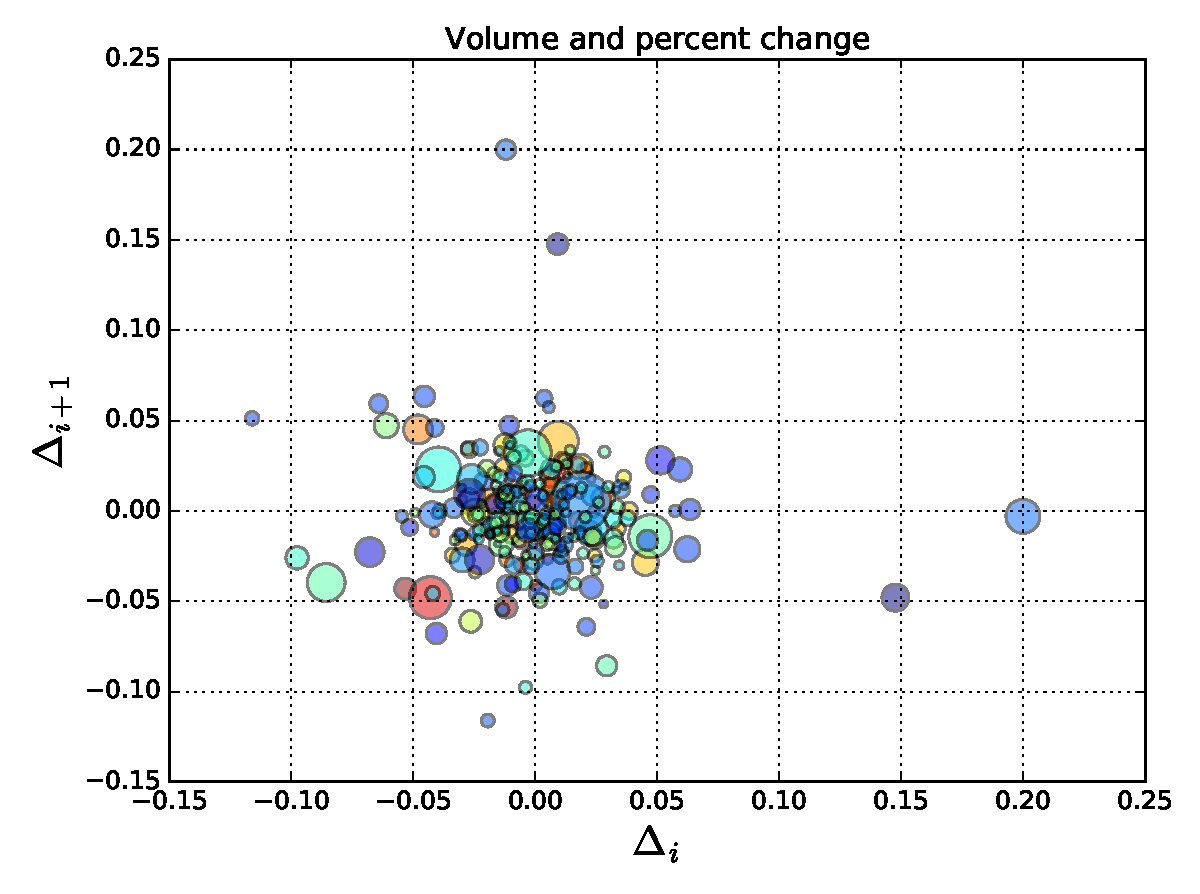
\includegraphics[width=15cm]{tabular-caption}
        \caption{一副图像}
    \end{center}
\end{figure}
